% =====================================================================
\chapter{System Design}
\label{ch:design}
% =====================================================================

This chapter specifies the \veriscript{} software system that implements the
methodology of Chapter~\ref{ch:proposed}. It begins with the functional and
non-functional requirements and the data flow diagrams, continues with
structural and dynamic models in the Unified Modeling Language (UML), and ends
with a detailed block diagram, the module interfaces and the external
application programming interface.

% ---------------------------------------------------------------------
\section{Functional Specification of the System}
% ---------------------------------------------------------------------

\subsection{Functional Requirements}

Table~\ref{tab:fr} lists the functional requirements. Each is traced to the
objective it serves.

\begin{table}[H]
\caption{Functional requirements of VeriScript}
\label{tab:fr}
\centering
\small
\begin{tabularx}{\textwidth}{|p{1.0cm}|L|p{1.5cm}|}
\hline
\textbf{ID} & \textbf{Requirement} & \textbf{Objective} \\ \hline
FR1 & Accept a single document as pasted text or as a .txt, .pdf or .docx file and extract its text. & O5 \\ \hline
FR2 & Accept a batch as a folder of files or a CSV file with \texttt{id} and \texttt{text} columns. & O5 \\ \hline
FR3 & Reject or flag documents shorter than the minimum length with the message ``insufficient text''. & O3 \\ \hline
FR4 & Compute the sixteen heuristic features and the calibrated probability $p_h(d)$. & O1 \\ \hline
FR5 & Route each document through the confidence gate using the configured band $[\Tlow,\Thigh]$. & O3 \\ \hline
FR6 & Run the fine-tuned transformer on escalated documents, with sliding windows for long texts. & O2 \\ \hline
FR7 & Return the label, calibrated probability, route and per-stage latency for every document. & O3, O4 \\ \hline
FR8 & Return an explanation listing the top contributing features for each decision. & O1, O3 \\ \hline
FR9 & Allow an administrator to choose an operating point (fast, balanced, thorough) or set custom thresholds. & O3 \\ \hline
FR10 & Produce a batch report (CSV and JSON) with per-document results and summary statistics. & O5 \\ \hline
FR11 & Provide an evaluation mode that computes accuracy, efficiency and fairness metrics on a labelled set. & O4 \\ \hline
FR12 & Allow retraining of the heuristic head and recalibration of the gate on new labelled data. & O1, O3 \\ \hline
\end{tabularx}
\end{table}

\subsection{Non-Functional Requirements}

\begin{table}[H]
\caption{Non-functional requirements of VeriScript}
\label{tab:nfr}
\centering
\small
\begin{tabularx}{\textwidth}{|p{1.0cm}|p{2.8cm}|L|}
\hline
\textbf{ID} & \textbf{Attribute} & \textbf{Requirement} \\ \hline
NFR1 & Performance & Average per-document latency of the cascade substantially below the transformer-only detector on the same CPU (target: at least 50\% lower). \\ \hline
NFR2 & Hardware & Must run on a CPU-only machine with 8 GB RAM; GPU used automatically when present. \\ \hline
NFR3 & Privacy & Documents are processed locally and are not stored unless the user enables logging. \\ \hline
NFR4 & Explainability & Every fast-path decision is accompanied by feature-level evidence. \\ \hline
NFR5 & Reproducibility & Fixed random seeds, versioned models and configuration files; evaluation runs are repeatable. \\ \hline
NFR6 & Modularity & Stages communicate through fixed interfaces so that either model can be replaced independently. \\ \hline
NFR7 & Usability & A non-technical user can check a document through the web interface in three steps. \\ \hline
NFR8 & Openness & Built only on open-source libraries and openly licensed model weights. \\ \hline
\end{tabularx}
\end{table}

\subsection{Level 0 Data Flow Diagram}

The context diagram in Fig.~\ref{fig:dfd0} treats \veriscript{} as a single
process. Three external entities interact with it: the \emph{reviewer}
(faculty member or moderator), who submits documents and receives results;
the \emph{administrator}, who configures operating points and supplies labelled
data for recalibration; and the \emph{model repository}, from which pretrained
weights are loaded.

\begin{figure}[H]
\centering
\begin{tikzpicture}
  \node[proc,minimum size=3.0cm] (sys) at (0,0) {\textbf{0.0}\\VeriScript\\detection\\system};
  \node[ext,minimum width=2.2cm] (rev) at (-5.6,0) {Reviewer};
  \node[ext,minimum width=2.2cm] (adm) at (5.6,0) {Administrator};
  \node[ext] (rep) at (0,-3.4) {Model repository};
  \draw[arr] ([yshift=0.3cm]rev.east) -- node[lbl,above,align=center] {documents,\\batch} ([yshift=0.3cm]rev.east -| sys.west);
  \draw[arr] ([yshift=-0.3cm]rev.east -| sys.west) -- node[lbl,below,align=center] {label, probability,\\explanation, report} ([yshift=-0.3cm]rev.east);
  \draw[arr] ([yshift=0.3cm]adm.west) -- node[lbl,above,align=center] {thresholds,\\labelled data} ([yshift=0.3cm]adm.west -| sys.east);
  \draw[arr] ([yshift=-0.3cm]adm.west -| sys.east) -- node[lbl,below,align=center] {metrics,\\status} ([yshift=-0.3cm]adm.west);
  \draw[arr] (rep) -- node[lbl,right] {model weights} (sys);
\end{tikzpicture}
\caption{Level 0 data flow diagram (context diagram)}
\label{fig:dfd0}
\end{figure}

\subsection{Level 1 Data Flow Diagram}

Fig.~\ref{fig:dfd1} decomposes the system into six processes and four data
stores. Process 1.0 extracts and normalises text; 2.0 computes heuristic
features and $p_h(d)$; 3.0 applies the gate; 4.0 runs the transformer on
escalated documents; 5.0 assembles the decision and explanation; and 6.0
calibrates and tunes thresholds from labelled data supplied by the
administrator. The data stores hold the calibrated heuristic model (D1), the
configuration with the current band (D2), the result log (D3) and the
fine-tuned transformer (D4).

\begin{figure}[H]
\centering
\resizebox{\textwidth}{!}{%
\begin{tikzpicture}[font=\small]
  % row 0: calibration path
  \node[ext] (adm) at (-7.0,5.8) {Administrator};
  \node[proc] (p6) at (-2.6,5.8) {6.0\\Calibrate and\\tune};
  \node[store,minimum width=2.9cm] (d1) at (0.9,5.8) {D1 \;Heuristic model};
  \node[store,minimum width=2.9cm] (d2) at (4.5,5.8) {D2 \;Configuration};
  % row 1: main path
  \node[ext] (rev) at (-7.0,2.3) {Reviewer};
  \node[proc] (p1) at (-2.6,2.3) {1.0\\Extract and\\pre-process};
  \node[proc] (p2) at (0.9,2.3) {2.0\\Heuristic\\scoring};
  \node[proc] (p3) at (4.5,2.3) {3.0\\Confidence\\gate};
  % row 2: decision
  \node[store,minimum width=2.6cm] (d3) at (-2.6,-1.2) {D3 \;Result log};
  \node[proc] (p5) at (0.9,-1.2) {5.0\\Decision and\\explanation};
  \node[proc] (p4) at (4.5,-1.2) {4.0\\Transformer\\inference};
  \node[store,minimum width=3.2cm] (d4) at (8.9,-1.2) {D4 \;Transformer model};
  % flows
  \draw[arr] (adm) -- node[lbl,above] {labelled data} (p6);
  \draw[arr] (p6) -- node[lbl,above] {calibrator} (d1);
  \draw[arr] (p6.north) to[bend left=22] node[lbl,above] {$\Tlow$, $\Thigh$} (d2.north);
  \draw[arr] (d1) -- node[lbl,right] {head} (p2);
  \draw[arr] (d2) -- node[lbl,right] {band} (p3);
  \draw[arr] (rev) -- node[lbl,above] {document} (p1);
  \draw[arr] (p1) -- node[lbl,above] {clean text} (p2);
  \draw[arr] (p2) -- node[lbl,above] {$p_h$, $\mathbf{h}$} (p3);
  \draw[arr] (p3) -- node[lbl,right] {escalated text} (p4);
  \draw[arr] (p3) -- node[lbl,above,sloped] {confident $p_h$} (p5);
  \draw[arr] (p4) -- node[lbl,above] {$p_t$} (p5);
  \draw[arr] (d4) -- node[lbl,above] {encoder} (p4);
  \draw[arr] (p5) -- node[lbl,above] {record} (d3);
  \draw[arr] (p5.south) .. controls (0.9,-3.4) and (-7.0,-3.4) .. node[lbl,below,pos=0.5] {result, explanation, report} (rev.south);
\end{tikzpicture}}
\caption{Level 1 data flow diagram}
\label{fig:dfd1}
\end{figure}

\subsection{Level 2 Data Flow Diagram for Heuristic Scoring}

Process 2.0 is the core of the fast path and is decomposed further in
Fig.~\ref{fig:dfd2}. The clean text is tokenised and passed once through the
reference model (2.1); token statistics are aggregated into perplexity, rank
and entropy features (2.2); sentence statistics give burstiness (2.3);
text-only analysis gives stylometric features (2.4); and the assembled vector
is standardised, scored by the head and calibrated (2.5).

\begin{figure}[H]
\centering
\resizebox{\textwidth}{!}{%
\begin{tikzpicture}[font=\small]
  \node[blk,text width=2.6cm] (in) at (-5.4,0) {Clean text\\(from 1.0)};
  \node[proc,minimum size=2.0cm] (a) at (-2.0,1.9) {2.1\\Reference\\LM pass};
  \node[proc,minimum size=2.0cm] (b) at (1.6,1.9) {2.2\\Token\\statistics};
  \node[proc,minimum size=2.0cm] (c) at (-2.0,-1.9) {2.3\\Sentence\\burstiness};
  \node[proc,minimum size=2.0cm] (dd) at (1.6,-1.9) {2.4\\Stylometric\\analysis};
  \node[proc,minimum size=2.0cm] (e) at (5.0,0) {2.5\\Scale, score,\\calibrate};
  \node[blk,text width=2.2cm] (out) at (8.0,0) {$p_h(d)$, $\mathbf{h}(d)$\\(to 3.0)};
  \draw[arr] (in) -- node[lbl,above,sloped] {tokens} (a);
  \draw[arr] (in) -- node[lbl,below,sloped] {sentences} (c);
  \draw[arr] (in.south) |- node[lbl,below,pos=0.75] {words, POS tags} (dd.south west);
  \draw[arr] (a) -- node[lbl,above] {log-probs, ranks} (b);
  \draw[arr] (a) -- node[lbl,left] {sentence PPL} (c);
  \draw[arr] (b) -- node[lbl,above,sloped] {features 1--9} (e);
  \draw[arr] (c.south) -- ++(0,-1.0) -| node[lbl,below,pos=0.25] {features 10--11} (e.south);
  \draw[arr] (dd) -- node[lbl,above,sloped] {12--16} (e);
  \draw[arr] (e) -- (out);
\end{tikzpicture}}
\caption{Level 2 data flow diagram for process 2.0 (heuristic scoring)}
\label{fig:dfd2}
\end{figure}

% ---------------------------------------------------------------------
\section{Structural and Dynamic Modeling of the System}
% ---------------------------------------------------------------------

\subsection{Class Diagram}

Fig.~\ref{fig:class} shows the main classes. \texttt{CascadeDetector} is the
facade used by both interfaces; it owns a \texttt{Preprocessor}, a
\texttt{HeuristicDetector} and a \texttt{TransformerDetector}, and delegates
the routing decision to a \texttt{ConfidenceGate}. The two detectors share a
common \texttt{Detector} interface with a \texttt{predict\_proba} method, which
is what allows either stage to be replaced (NFR6). Each call returns a
\texttt{DetectionResult} that contains an \texttt{Explanation}.

\tikzset{
  umlclass/.style={draw,thick,rectangle split,rectangle split parts=3,
     rectangle split part align={center,left,left},
     font=\scriptsize,inner sep=3pt,text width=4.0cm,fill=white},
}
\begin{figure}[H]
\centering
\begin{tikzpicture}[node distance=0.7cm and 0.6cm]
  \node[umlclass] (cd) at (0,0) {\textbf{CascadeDetector}
     \nodepart{second} -- t\_low: float\\ -- t\_high: float\\ -- tau: float
     \nodepart{third} + detect(text): DetectionResult\\ + detect\_batch(docs): List\\ + set\_operating\_point(name)};
  \node[umlclass] (pre) at (-5.0,0) {\textbf{Preprocessor}
     \nodepart{second} -- min\_words: int
     \nodepart{third} + clean(text): str\\ + sentences(text): List\\ + is\_sufficient(text): bool};
  \node[umlclass] (gate) at (5.0,0) {\textbf{ConfidenceGate}
     \nodepart{second} -- t\_low: float\\ -- t\_high: float
     \nodepart{third} + route(p\_h): Route\\ + tune(val\_preds, eps, delta)};
  \node[umlclass,text width=3.4cm] (det) at (0,-3.7) {\textbf{$\ll$interface$\gg$ Detector}
     \nodepart{second} \;
     \nodepart{third} + predict\_proba(text): float\\ + latency(): float};
  \node[umlclass] (heu) at (-4.4,-6.9) {\textbf{HeuristicDetector}
     \nodepart{second} -- extractor: FeatureExtractor\\ -- head: LR | GBDT\\ -- calibrator: Calibrator
     \nodepart{third} + predict\_proba(text): float\\ + explain(h, k): Explanation};
  \node[umlclass] (tra) at (4.4,-6.9) {\textbf{TransformerDetector}
     \nodepart{second} -- model\_name: str\\ -- max\_len: int = 512\\ -- stride: int = 384
     \nodepart{third} + predict\_proba(text): float\\ + windows(text): List};
  \node[umlclass] (fe) at (-4.4,-10.6) {\textbf{FeatureExtractor}
     \nodepart{second} -- ref\_lm: GPT-2 small\\ -- scaler: StandardScaler
     \nodepart{third} + extract(text): Vector\\ + names(): List[str]};
  \node[umlclass] (res) at (4.4,-10.6) {\textbf{DetectionResult}
     \nodepart{second} -- label: int\\ -- probability: float\\ -- route: Route\\ -- latency\_ms: dict
     \nodepart{third} + to\_json(): dict};
  \node[umlclass,text width=3.0cm] (exp) at (4.4,-13.6) {\textbf{Explanation}
     \nodepart{second} -- top\_features: List\\ -- note: str
     \nodepart{third} + render(): str};
  % associations
  \draw[thick] (cd.west) -- node[lbl,above] {uses} (pre.east);
  \draw[thick] (cd.east) -- node[lbl,above] {uses} (gate.west);
  \draw[thick,-{Triangle[open,length=3mm]},dashed] (heu.north) |- ([yshift=-4pt]det.west);
  \draw[thick,-{Triangle[open,length=3mm]},dashed] (tra.north) |- ([yshift=-4pt]det.east);
  \draw[thick,{Diamond[length=3mm]}-] (cd.south) -- node[lbl,right] {1..2} (det.north);
  \draw[thick,{Diamond[length=3mm]}-] (heu.south) -- node[lbl,right] {1} (fe.north);
  \draw[thick,->] (cd.south east) to[out=-40,in=60] node[lbl,right,pos=0.4] {creates} (res.north east);
  \draw[thick,{Diamond[length=3mm]}-] (res.south) -- node[lbl,right] {1} (exp.north);
\end{tikzpicture}
\caption{Class diagram of the VeriScript core library}
\label{fig:class}
\end{figure}

\subsection{Use Case Diagram}

Fig.~\ref{fig:usecase} shows the actors and use cases. The \emph{reviewer}
checks single documents, uploads batches, inspects explanations and downloads
reports. The \emph{administrator} configures operating points, recalibrates the
gate and runs evaluations. The \emph{researcher} retrains models and runs the
benchmark evaluation. ``Run cascade detection'' is included by both checking
use cases, and ``View explanation'' extends the result view.

\tikzset{usecase/.style={draw,thick,ellipse,align=center,font=\footnotesize,
          minimum width=3.6cm,minimum height=0.9cm,inner sep=1pt}}
\newcommand{\stickman}[2]{%
  \begin{scope}[shift={(#1)},thick]
    \draw (0,0.55) circle (0.2);
    \draw (0,0.35) -- (0,-0.25);
    \draw (-0.35,0.15) -- (0.35,0.15);
    \draw (0,-0.25) -- (-0.25,-0.7) (0,-0.25) -- (0.25,-0.7);
    \node[below,font=\small] at (0,-0.75) {#2};
  \end{scope}}
\begin{figure}[H]
\centering
\begin{tikzpicture}
  \draw[thick] (-3.0,-5.6) rectangle (3.4,4.6);
  \node[font=\small\bfseries] at (0.2,4.25) {VeriScript system};
  \node[usecase] (u1) at (0.2,3.4) {Check single document};
  \node[usecase] (u2) at (0.2,2.2) {Upload batch};
  \node[usecase] (u3) at (0.2,1.0) {Run cascade detection};
  \node[usecase] (u4) at (0.2,-0.2) {View result};
  \node[usecase] (u5) at (0.2,-1.4) {View explanation};
  \node[usecase] (u6) at (0.2,-2.6) {Download report};
  \node[usecase] (u7) at (0.2,-3.7) {Configure operating point};
  \node[usecase] (u8) at (0.2,-4.8) {Recalibrate / run evaluation};
  \stickman{-5.3,1.3}{Reviewer}
  \stickman{5.6,-2.9}{Administrator}
  \stickman{5.6,1.6}{Researcher}
  \foreach \u in {u1,u2,u4,u6} \draw[thick] (-4.95,1.3) -- (\u.west);
  \foreach \u in {u7,u8} \draw[thick] (5.25,-2.9) -- (\u.east);
  \draw[thick] (5.25,1.6) -- (u8.east);
  \draw[thick] (5.25,1.6) -- (u3.east);
  \draw[->,dashed] (u1.east) to[out=-20,in=20] node[lbl,right,font=\tiny] {$\ll$include$\gg$} (u3.east);
  \draw[->,dashed] (u2) -- node[lbl,right,font=\tiny] {$\ll$include$\gg$} (u3);
  \draw[->,dashed] (u5) -- node[lbl,right,font=\tiny] {$\ll$extend$\gg$} (u4);
\end{tikzpicture}
\caption{Use case diagram}
\label{fig:usecase}
\end{figure}

\subsection{Interaction (Sequence) Diagram}

Fig.~\ref{fig:sequence} shows the interaction for checking one document. The
first part is common to all documents. The \texttt{alt} fragment then shows the
two alternatives: on the fast path the heuristic detector supplies the
explanation; on the escalated path the transformer detector is called and its
probability replaces the heuristic one.

\begin{figure}[H]
\centering
\resizebox{\textwidth}{!}{%
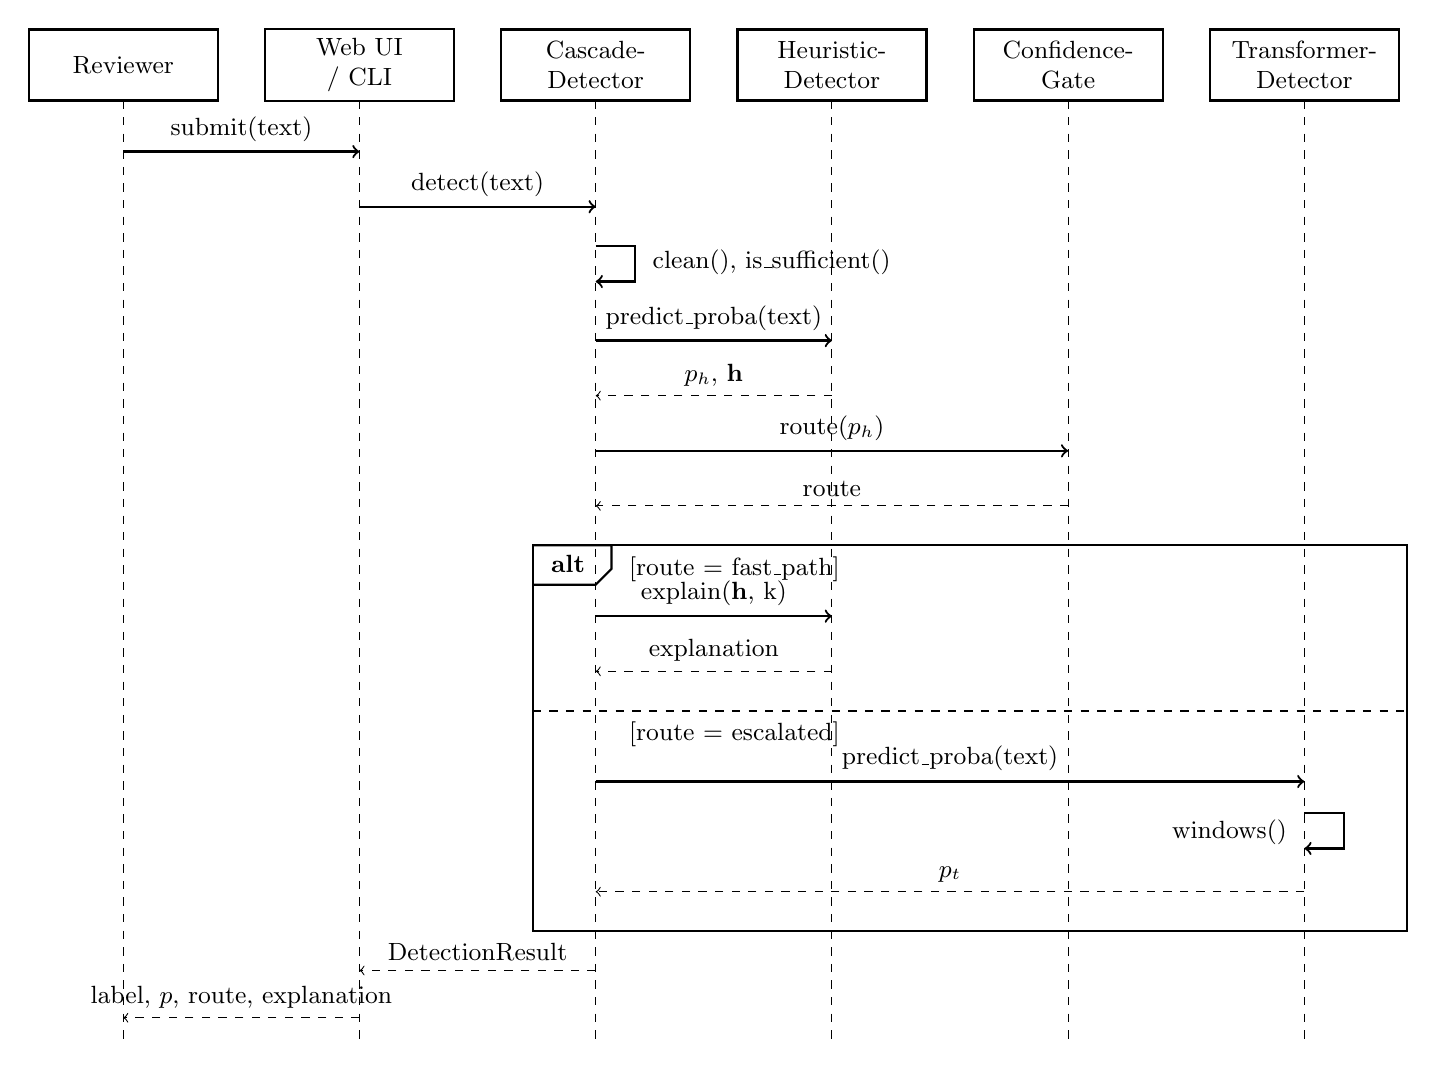
\begin{tikzpicture}[font=\small]
  \foreach \x/\name/\id in {0/Reviewer/r,3/{Web UI\\/ CLI}/ui,6/Cascade-\\Detector/cd,
                            9/Heuristic-\\Detector/hd,12/Confidence-\\Gate/g,15/Transformer-\\Detector/td}{
     \node[draw,thick,fill=white,minimum width=2.4cm,minimum height=0.9cm,align=center] (\id) at (\x,0) {\name};
     \draw[dashed] (\x,-0.45) -- (\x,-12.4);
  }
  \newcommand{\msg}[4]{\draw[->,thick] (#1,#3) -- node[above] {#4} (#2,#3);}
  \newcommand{\ret}[4]{\draw[->,dashed] (#1,#3) -- node[above] {#4} (#2,#3);}
  \msg{0}{3}{-1.1}{submit(text)}
  \msg{3}{6}{-1.8}{detect(text)}
  \draw[->,thick] (6,-2.3) -- ++(0.5,0) -- ++(0,-0.45) -- ++(-0.5,0);
  \node[anchor=west] at (6.6,-2.5) {clean(), is\_sufficient()};
  \msg{6}{9}{-3.5}{predict\_proba(text)}
  \ret{9}{6}{-4.2}{$p_h$, $\mathbf{h}$}
  \msg{6}{12}{-4.9}{route($p_h$)}
  \ret{12}{6}{-5.6}{route}
  % alt frame
  \draw[thick] (5.2,-6.1) rectangle (16.3,-11.0);
  \draw[thick] (5.2,-6.1) -- ++(1.0,0) -- ++(0,-0.3) -- ++(-0.2,-0.2) -- (5.2,-6.6);
  \node[font=\small\bfseries] at (5.65,-6.33) {alt};
  \node[anchor=west] at (6.3,-6.4) {[route = fast\_path]};
  \msg{6}{9}{-7.0}{explain($\mathbf{h}$, k)}
  \ret{9}{6}{-7.7}{explanation}
  \draw[dashed,thick] (5.2,-8.2) -- (16.3,-8.2);
  \node[anchor=west] at (6.3,-8.5) {[route = escalated]};
  \msg{6}{15}{-9.1}{predict\_proba(text)}
  \draw[->,thick] (15,-9.5) -- ++(0.5,0) -- ++(0,-0.45) -- ++(-0.5,0);
  \node[anchor=east] at (14.9,-9.75) {windows()};
  \ret{15}{6}{-10.5}{$p_t$}
  \ret{6}{3}{-11.5}{DetectionResult}
  \ret{3}{0}{-12.1}{label, $p$, route, explanation}
\end{tikzpicture}}
\caption{Sequence diagram for checking a single document}
\label{fig:sequence}
\end{figure}

\subsection{Activity Diagram}

Fig.~\ref{fig:activity} shows the activity of batch processing. Documents are
processed in a loop. The heuristic stage runs for every document; escalated
documents are collected and passed to the transformer in mini-batches, which
uses the hardware more efficiently than one document at a time. The report is
written once all documents are processed.

\begin{figure}[H]
\centering
\begin{tikzpicture}[node distance=0.5cm and 0.8cm,font=\small]
  \node[circle,fill=black,minimum size=0.35cm] (s) {};
  \node[term,below=of s] (a1) {Load batch and configuration};
  \node[term,below=of a1] (a2) {Take next document};
  \node[term,below=of a2] (a3) {Pre-process and check length};
  \node[dec,below=of a3] (d1) {Sufficient?};
  \node[term,right=1.0cm of d1] (a4) {Mark ``insufficient''};
  \node[term,below=of d1] (a5) {Heuristic scoring $p_h$};
  \node[dec,below=of a5] (d2) {In band?};
  \node[term,left=1.0cm of d2] (a6) {Record fast-path result};
  \node[term,right=1.0cm of d2] (a7) {Add to escalation queue};
  \node[dec,below=1.3cm of d2] (d3) {More docs?};
  \node[term,below=of d3] (a8) {Transformer on queue (mini-batches)};
  \node[term,below=of a8] (a9) {Write CSV/JSON report and summary};
  \node[circle,draw,thick,minimum size=0.45cm,below=of a9] (e) {};
  \node[circle,fill=black,minimum size=0.28cm] at (e) {};
  \draw[arr] (s) -- (a1);
  \draw[arr] (a1) -- (a2);
  \draw[arr] (a2) -- (a3);
  \draw[arr] (a3) -- (d1);
  \draw[arr] (d1) -- node[lbl,above] {no} (a4);
  \draw[arr] (d1) -- node[lbl,right] {yes} (a5);
  \draw[arr] (a5) -- (d2);
  \draw[arr] (d2) -- node[lbl,above] {no} (a6);
  \draw[arr] (d2) -- node[lbl,above] {yes} (a7);
  \draw[arr] (a6) |- (d3);
  \draw[arr] (a7) |- (d3);
  \draw[arr] (a4.east) -- ++(0.6,0) |- (d3.east);
  \draw[arr] (d3.west) -- node[lbl,above,pos=0.15] {yes} ++(-4.9,0) |- (a2.west);
  \draw[arr] (d3) -- node[lbl,right] {no} (a8);
  \draw[arr] (a8) -- (a9);
  \draw[arr] (a9) -- (e);
\end{tikzpicture}
\caption{Activity diagram for batch processing}
\label{fig:activity}
\end{figure}

\subsection{State Chart Diagram}

Fig.~\ref{fig:state} gives the life cycle of a detection job for one
document. A job begins in the \emph{Received} state and ends in
\emph{Reported}. The \emph{Escalated} state exists only for documents in the
ambiguity band, and \emph{Rejected} covers inputs that are too short or whose
text cannot be extracted.

\begin{figure}[H]
\centering
\begin{tikzpicture}[
   st/.style={draw,thick,rounded corners=6pt,minimum width=2.6cm,minimum height=0.9cm,align=center,font=\small}]
  \node[circle,fill=black,minimum size=0.35cm] (init) at (-2.2,0) {};
  \node[st] (rec) at (0,0) {Received};
  \node[st] (pre) at (4.0,0) {Pre-processing};
  \node[st] (rej) at (9.0,0) {Rejected};
  \node[st] (hs) at (4.0,-2.3) {Heuristic\\scored};
  \node[st] (dec) at (1.4,-4.6) {Decided};
  \node[st] (esc) at (6.4,-4.6) {Escalated};
  \node[st] (rep) at (1.4,-6.9) {Reported};
  \node[circle,draw,thick,minimum size=0.5cm] (fin) at (9.0,-6.9) {};
  \node[circle,fill=black,minimum size=0.3cm] at (fin) {};
  \draw[arr] (init) -- (rec);
  \draw[arr] (rec) -- node[lbl,above] {start} (pre);
  \draw[arr] (pre) -- node[lbl,above,yshift=2pt] {too short / unreadable} (rej);
  \draw[arr] (pre) -- node[lbl,right] {text ready} (hs);
  \draw[arr] (hs) -- node[lbl,above,sloped] {$p_h \notin$ band} (dec);
  \draw[arr] (hs) -- node[lbl,above,sloped] {$p_h \in$ band} (esc);
  \draw[arr] (esc) -- node[lbl,above] {$p_t$ computed} (dec);
  \draw[arr] (dec) -- node[lbl,right] {explanation added} (rep);
  \draw[arr] (rej) -- node[lbl,right] {error reported} (fin);
  \draw[arr] (rep) -- node[lbl,above] {result delivered} (fin);
\end{tikzpicture}
\caption{State chart diagram of a detection job}
\label{fig:state}
\end{figure}

\subsection{Component and Deployment Diagrams}

Fig.~\ref{fig:component} shows the software components. The \texttt{veriscript-core}
library contains the pre-processing, feature, model, gate and explanation
modules and has no dependency on any user interface. Three thin front ends use
it: the command line tool, a REST service built with FastAPI, and a web
interface that calls the REST service. The evaluation toolkit uses the same
core library, which guarantees that what is evaluated is exactly what is
deployed.

\begin{figure}[H]
\centering
\begin{tikzpicture}[font=\small,
  comp/.style={draw,thick,minimum width=3.0cm,minimum height=1.0cm,align=center,fill=white,
    append after command={
      \pgfextra{\draw[thick,fill=white] ($(\tikzlastnode.north east)+(-0.45,-0.15)$) rectangle ++(0.3,-0.3);
                \draw[thick,fill=white] ($(\tikzlastnode.north east)+(-0.52,-0.2)$) rectangle ++(0.14,-0.07);
                \draw[thick,fill=white] ($(\tikzlastnode.north east)+(-0.52,-0.33)$) rectangle ++(0.14,-0.07);}}}]
  \node[comp] (cli) at (-4.4,3.0) {CLI\\(\texttt{veriscript})};
  \node[comp] (api) at (0,3.0) {REST service\\(FastAPI)};
  \node[comp] (web) at (4.4,3.0) {Web interface};
  \node[comp] (evl) at (-4.4,-2.6) {Evaluation\\toolkit};
  \draw[thick] (-3.6,-1.6) rectangle (3.6,1.8);
  \node[font=\small\bfseries,anchor=north west] at (-3.55,1.75) {veriscript-core};
  \tikzset{mod/.style={draw,thick,rounded corners=2pt,font=\scriptsize,align=center,
           text width=1.8cm,minimum height=0.7cm,inner sep=2pt}}
  \node[mod] (m1) at (-2.3,0.5) {preprocess};
  \node[mod] (m2) at (0,0.5) {features +\\heuristic};
  \node[mod] (m3) at (2.3,0.5) {gate +\\cascade};
  \node[mod] (m4) at (-1.15,-0.8) {transformer};
  \node[mod] (m5) at (1.15,-0.8) {explain};
  \node[store,minimum width=2.6cm] (ms) at (1.8,-3.0) {Model store};
  \node[store,minimum width=2.6cm] (cf) at (5.4,-0.6) {Config (YAML)};
  \draw[arr,dashed] (cli) -- (cli |- 0,1.8);
  \draw[arr,dashed] (api) -- (0,1.8);
  \draw[arr,dashed] (web) -- node[lbl,above] {HTTP/JSON} (api);
  \draw[arr,dashed] (evl) -- (evl |- 0,-1.6);
  \draw[arr,dashed] (ms |- 0,-1.6) -- (ms);
  \draw[arr,dashed] (3.6,-0.6) -- (cf.west);
\end{tikzpicture}
\caption{Component diagram}
\label{fig:component}
\end{figure}

Fig.~\ref{fig:deployment} shows the deployment. The system runs as a container
on an institutional server (CPU, with an optional GPU). Reviewers use a
browser on their own machines; staff who process large batches can install
the CLI on a workstation, which loads the same models locally.

\begin{figure}[H]
\centering
\resizebox{\textwidth}{!}{%
\begin{tikzpicture}[font=\small,
   node3d/.style={draw,thick,minimum width=4.2cm,minimum height=2.8cm,align=center,fill=white}]
  \newcommand{\cube}[3]{% name, position, label
    \node[node3d] (#1) at (#2) {};
    \draw[thick] (#1.north west) -- ++(0.3,0.3) -- ($(#1.north east)+(0.3,0.3)$) -- (#1.north east);
    \draw[thick] ($(#1.north east)+(0.3,0.3)$) -- ($(#1.south east)+(0.3,0.3)$) -- (#1.south east);
    \node[font=\small,anchor=north,align=center] at ([yshift=-3pt]#1.north) {#3};}
  \cube{client}{-5.4,0}{$\ll$device$\gg$\\\textbf{Reviewer PC}}
  \node[draw,font=\small,align=center] at ($(client.center)+(0,-0.6)$) {Web browser};
  \cube{server}{0.4,0}{$\ll$device$\gg$\\\textbf{Institution server}}
  \node[draw,font=\footnotesize,align=center,text width=3.5cm] at ($(server.center)+(0,-0.6)$) {Docker container: FastAPI, web UI, core, models};
  \cube{ws}{0.4,-4.6}{$\ll$device$\gg$\\\textbf{Staff workstation}}
  \node[draw,font=\small,align=center] at ($(ws.center)+(0,-0.6)$) {CLI + core + models};
  \cube{gpu}{6.2,0}{$\ll$optional device$\gg$\\\textbf{GPU}}
  \node[font=\small,align=center] at ($(gpu.center)+(0,-0.6)$) {CUDA runtime};
  \draw[thick] (client.east) -- node[lbl,above] {HTTPS} (server.west);
  \draw[thick] ([xshift=0.3cm]server.east) -- node[lbl,above] {PCIe} (gpu.west);
  \draw[thick,dashed] (server.south) -- node[lbl,right] {model files} (ws.north);
\end{tikzpicture}}
\caption{Deployment diagram}
\label{fig:deployment}
\end{figure}

% ---------------------------------------------------------------------
\section{Detailed Block Diagram}
% ---------------------------------------------------------------------

Fig.~\ref{fig:detailblock} brings the design together as a detailed block
diagram of the run-time pipeline, showing the data that passes between the
modules and the measurement points used by the evaluation.

\begin{figure}[H]
\centering
\begin{tikzpicture}[node distance=0.5cm and 0.5cm,font=\small]
  \node[io,text width=3.2cm] (in) {Input: text / file / batch};
  \node[blk,below=of in,text width=4.2cm] (ex) {Text extraction\\(pdfplumber, python-docx)};
  \node[blk,below=of ex,text width=4.2cm] (pp) {Pre-processing: NFKC, whitespace, markup removal, sentence split (spaCy)};
  \node[blk,below=of pp,text width=4.2cm] (lm) {Reference LM pass\\GPT-2 small, one forward pass};
  \node[blk,below=of lm,text width=4.2cm] (fv) {Feature vector $\mathbf{h}(d)$ (16 features) + standardisation};
  \node[blk,below=of fv,text width=4.2cm] (hd) {LR / GBDT head + calibrator $\rightarrow p_h(d)$};
  \node[dec,below=0.6cm of hd] (gt) {Gate};
  \node[blk,right=1.4cm of hd,text width=3.6cm] (tok) {Tokeniser + sliding windows ($L$=512, stride 384)};
  \node[blk,above=of tok,text width=3.6cm] (enc) {RoBERTa-base / DeBERTa-v3 classifier};
  \node[blk,above=of enc,text width=3.6cm] (agg) {Window averaging $\rightarrow p_t(d)$};
  \node[blk,below=1.0cm of gt,text width=4.2cm] (dc) {Decision $\hat{y}=\mathbb{1}[p\ge\tau]$ + explanation};
  \node[io,below=of dc,text width=3.6cm] (out) {Result JSON / report};
  \node[draw,dashed,thick,left=1.0cm of lm,text width=2.2cm,align=center,font=\scriptsize] (t1) {timer $t_h$ starts};
  \node[draw,dashed,thick,left=1.0cm of dc,text width=2.2cm,align=center,font=\scriptsize] (t2) {timers $t_h$, $t_t$ logged};
  \draw[arr] (in) -- (ex);
  \draw[arr] (ex) -- (pp);
  \draw[arr] (pp) -- (lm);
  \draw[arr] (lm) -- (fv);
  \draw[arr] (fv) -- (hd);
  \draw[arr] (hd) -- (gt);
  \draw[arr] (gt.east) -| node[lbl,below,pos=0.3] {escalate} (tok.south);
  \draw[arr] (tok) -- (enc);
  \draw[arr] (enc) -- (agg);
  \draw[arr] (agg.east) -- ++(0.5,0) |- node[lbl,right,pos=0.2] {$p_t$} (dc.east);
  \draw[arr] (gt) -- node[lbl,right] {fast path ($p_h$)} (dc);
  \draw[arr] (dc) -- (out);
  \draw[dotted,thick] (t1) -- (lm);
  \draw[dotted,thick] (t2) -- (dc);
\end{tikzpicture}
\caption{Detailed block diagram of the VeriScript run-time pipeline}
\label{fig:detailblock}
\end{figure}

\subsection{Module Interfaces}

Table~\ref{tab:modules} lists the modules of the core library with their
inputs and outputs. Fixed interfaces between modules satisfy NFR6 and allow
each module to be unit-tested independently.

\begin{table}[H]
\caption{Modules of the VeriScript core library}
\label{tab:modules}
\centering
\small
\begin{tabularx}{\textwidth}{|p{2.8cm}|L|L|}
\hline
\textbf{Module} & \textbf{Input} & \textbf{Output} \\ \hline
\texttt{io.extract} & File path or raw text & UTF-8 plain text \\ \hline
\texttt{preprocess} & Plain text & Clean text, sentence list, word count \\ \hline
\texttt{features} & Clean text, sentence list & 16-dimensional feature vector with names \\ \hline
\texttt{heuristic} & Feature vector & Calibrated $p_h(d)$; feature contributions \\ \hline
\texttt{gate} & $p_h(d)$, band & Route (\texttt{fast\_path} / \texttt{escalated}) \\ \hline
\texttt{transformer} & Clean text & $p_t(d)$, number of windows \\ \hline
\texttt{explain} & Contributions, route, probabilities & Explanation object \\ \hline
\texttt{cascade} & Text or list of texts & \texttt{DetectionResult} objects \\ \hline
\texttt{evaluate} & Labelled dataset, system name & Metrics table, plots, fairness report \\ \hline
\end{tabularx}
\end{table}

\subsection{External Interface (REST API)}

The REST service exposes the endpoints in Table~\ref{tab:api}. All responses
are JSON. Batch jobs are processed asynchronously so that the web interface
remains responsive.

\begin{table}[H]
\caption{REST API endpoints}
\label{tab:api}
\centering
\small
\begin{tabularx}{\textwidth}{|p{1.4cm}|p{3.6cm}|L|}
\hline
\textbf{Method} & \textbf{Endpoint} & \textbf{Description} \\ \hline
POST & \texttt{/api/v1/detect} & Detect a single document; body \texttt{\{"text": ...\}}; returns label, probability, route, latency, explanation \\ \hline
POST & \texttt{/api/v1/batch} & Submit a batch (CSV or ZIP); returns a job identifier \\ \hline
GET & \texttt{/api/v1/batch/\{id\}} & Job status and, when complete, the report \\ \hline
GET & \texttt{/api/v1/config} & Current operating point and thresholds \\ \hline
PUT & \texttt{/api/v1/config} & Change operating point (administrator only) \\ \hline
GET & \texttt{/api/v1/health} & Service and model status \\ \hline
\end{tabularx}
\end{table}

A response produced by the implemented service for a 147-word AI-generated
test document (balanced operating point, GPU) is shown below; the list of
features is shortened to three entries.
\begin{lstlisting}[language={},numbers=none,caption={JSON response of the detect endpoint for a fast-path decision},label={lst:json}]
{
  "label": "ai_generated",
  "probability": 1.0,
  "route": "fast_path",
  "latency_ms": {"heuristic": 40.1, "transformer": 0.0, "total": 48.02},
  "n_words": 147,
  "explanation": {
    "top_features": [
      {"name": "mean_log_prob", "value": -2.4165,
       "human_median": -3.4925, "ai_median": -2.314},
      {"name": "perplexity", "value": 11.2062,
       "human_median": 32.868, "ai_median": 10.1148},
      {"name": "pos_bigram:NOUN_CCONJ", "value": 0.0513,
       "human_median": 0.0095, "ai_median": 0.0149}
    ],
    "note": "Probabilistic estimate; review before acting on it.",
    "decided_by": "heuristic",
    "heuristic_probability": 1.0,
    "transformer_probability": null,
    "n_windows": null
  }
}
\end{lstlisting}
Each feature is reported with the median value of that feature among the
human-written and AI-generated training documents, so that a reviewer can see
on which side of the typical ranges the document falls.

\section{Summary}

This chapter specified the requirements of \veriscript{} and modelled the
system at several levels: data flow diagrams from the context level to the
decomposition of heuristic scoring; class, use case, sequence, activity, state,
component and deployment diagrams; and a detailed block diagram with module
and API interfaces. The next chapter describes the implementation: the
algorithms and tools used, the experimental setup and the datasets.
